

%%%%
%%%%
%%%%
\chapter{Query compilation workflow}
%%%%
%%%%
%%%%

After the model handling code is generated, the user of the framework can build and maintain the live model at runtime. 
Still to use find matches for graph patterns, we need additional components to be generated. 
In this chapter, we show the workflow of query code generation in the framework. 


\begin{figure}[H]
	\begin{center}
		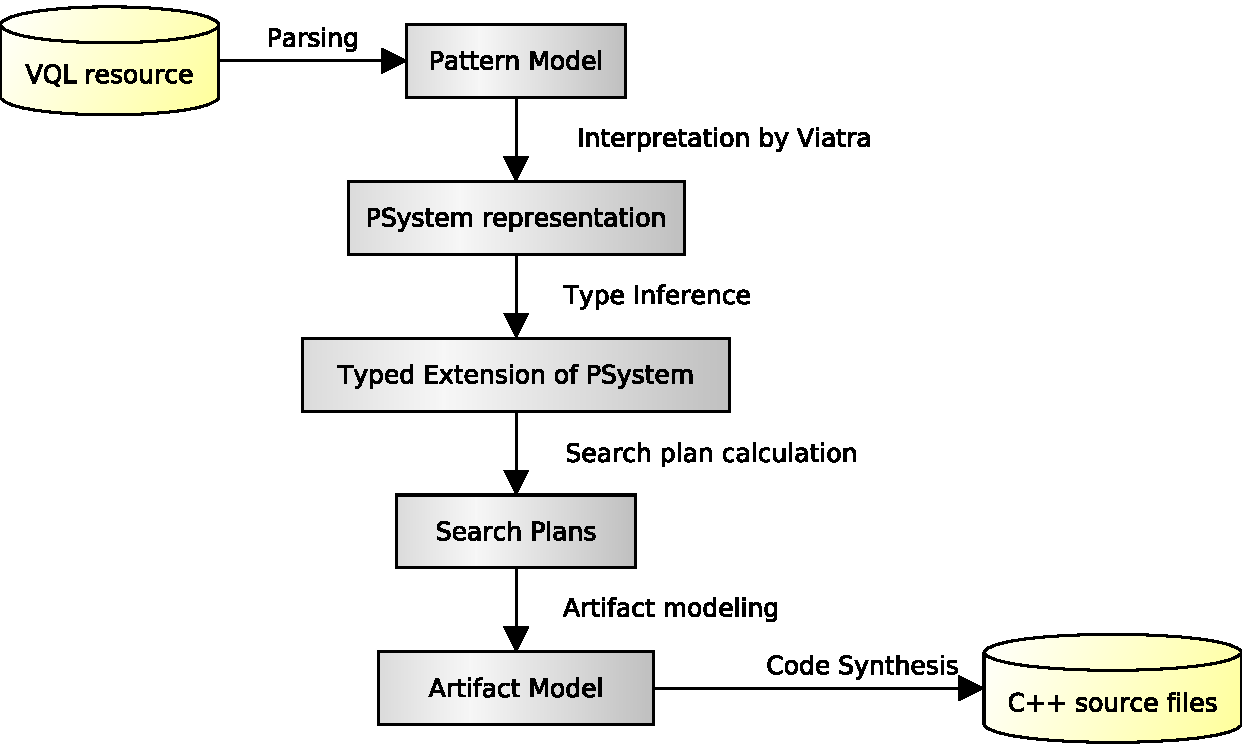
\includegraphics[width=\textwidth]{figures/query-compilation-workflow.pdf}
		\caption{Query compilation workflow}
		\label{figure:query-compile-workflow}
	\end{center}
\end{figure}


\section{Overview}

The compilation of graph patterns is depicted in fig. \ref{figure:query-compile-workflow}:

\begin{enumerate}[(1)]

\item 
First, VQL files containing the patterns are parsed using EMF so their contents are loaded into a Pattern Model.
\item 
The Pattern Model is processed by \viatra{} and converted into PSystem representation of queries.
\item 
After that, we extend this representation with type information, as type information is more important in the \cpp{} generated code, than in the \viatra{} implementation.
\item 
Then, we create the plan for query execution; we use the local search planner of \viatra{} fine tuned with our search operation cost function to improve performance of distributed queries. 
We also use some optimizations later to improve distributed performance. 
\item 
After the fully optimized plan is ready, we can construct the generator model describing the source code structure 
\item
and generate the \cpp{} files from them.

\end{enumerate}



\section{PSystem representation}


The VQL file is loaded into a PatternModel. 
The framework does not use this representation, but passes it to \viatra, which creates its own representations of it called PSystem. \cite{psystem}. 


\begin{figure}[H]
	\begin{center}
		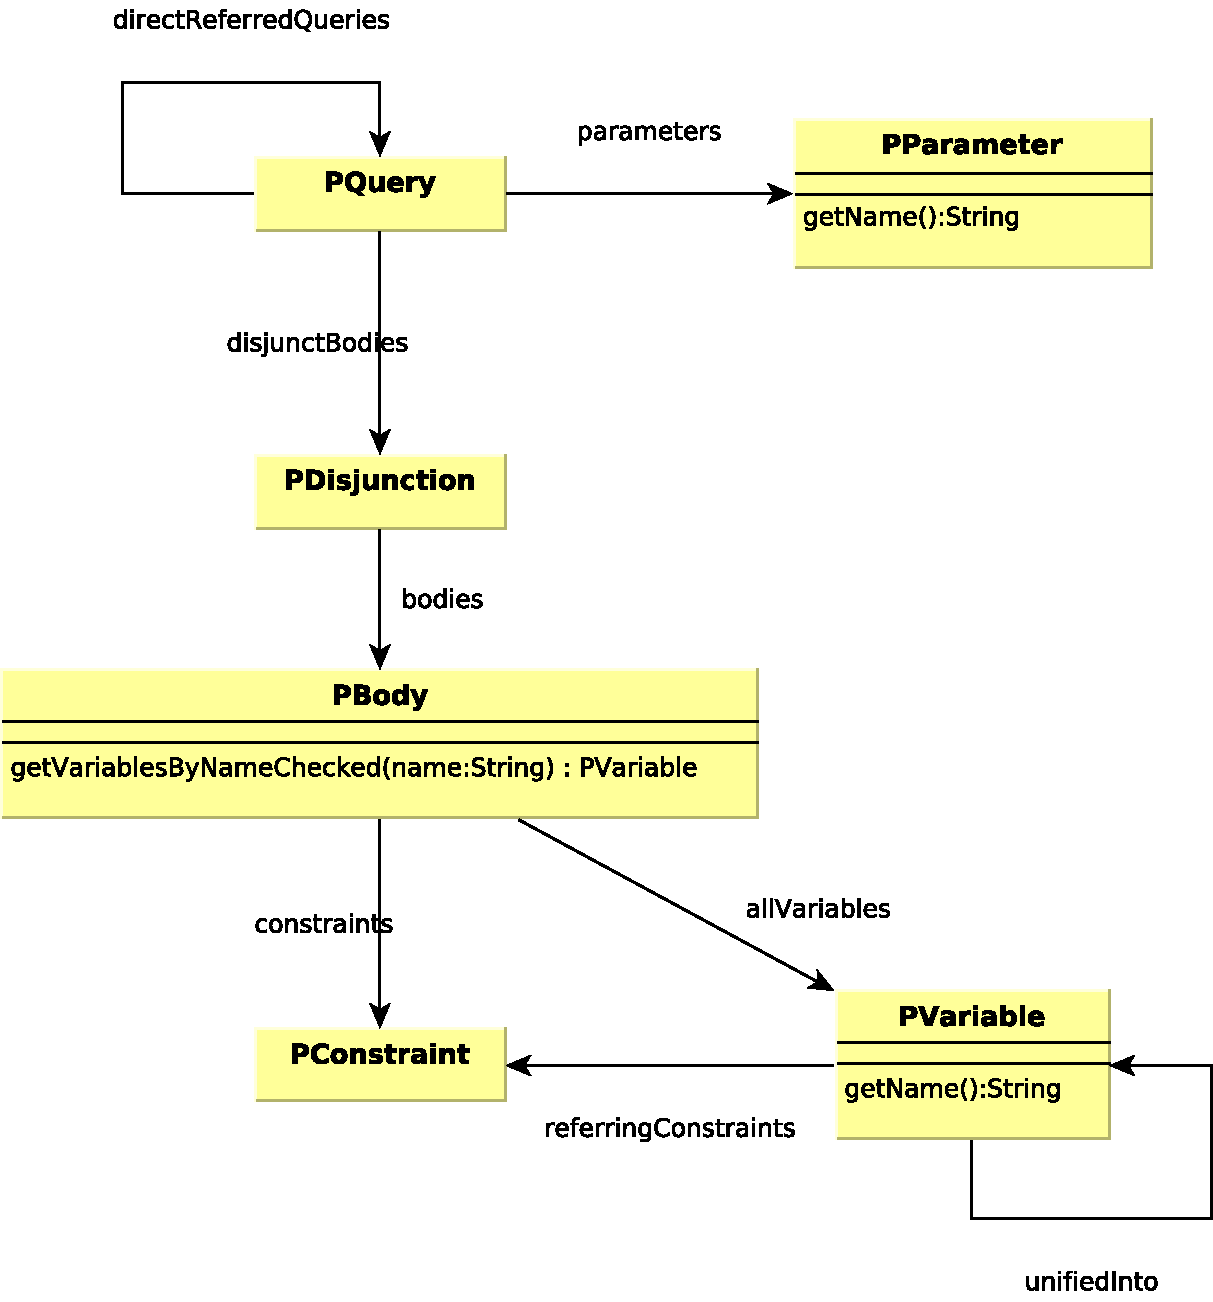
\includegraphics[width=0.6\textwidth]{figures/psystem.pdf}
		\caption{PSystem's basic structure}
		\label{fig:psystem}
	\end{center}
\end{figure}

The structure of PSystem representation is shown on \autoref{fig:psystem}. 
As their implementation is hidden behind interfaces, most of the refrences means getter functions (In Xtend, getter functions can be used with field access syntax like \csharp{} properties). 
Graph patterns are represented by a PQuery. 
A PQuery has a parameter list. 
The most important attribute of parameters are its names. 
A PQuery consists of a PDisjunction, which consists of a set of PBodies. 
PDisjunctions play role in Query rewriting, where the bodies of a PQuery gets optimized, or changed other ways.
PBody consists of PConstraints. 
PConstraint is a basic interface for various constraints. 
Altough constraints refer to variables, all variables in a PBody can be accessed from PBody.

%A variable can be unified into another variable. 
%This can happen when equality constraint is used between two variable: 
%Equality constraint is omitted, one of the variable gets unified into the other, and other constraints do not have to be changed.



\section{Typed Extension of PSystem}

We extend PSystem with additional information, mainly with type information for variables and parameters.
For this the types of the variables and parameters must be infered based on type constraints of the graph pattern.

First the types of the variables must be infered. 
\begin{enumerate}
	\item 
	First, we collect all the type constraints, that the variable must satisfy.
	We do this, by collecting all the variables that are the same as the variable( via equality constraints ), 
	then collect the constraints refering to them.
	From this we can create the set of candidate types.
	\item
	Then we choose the type:
	\begin{itemize}
		\item
		If all the types are compatible data types (integral types, or the same type), then we choose the most specific type
		\item
		If all the types are EClass types, then we select the most general class, that is compatible (extends it or is the same) of all the classes and choose that.
		If we cannot choose such EClass, or there are multiple classes that satisfies this, then the type inference is failed.
		A case for this is depicted on \autoref{fig:multiple-inheritance-problem}: if a variable's type is restricted as \texttt{A} and \texttt{B}, we cannot choose between \texttt{X} and \texttt{Y}
		\item
		In other cases (e.g. both of data types and class types is used) the type inference is failed
	\end{itemize}
\end{enumerate}


\begin{figure}[h]
	\begin{center}
		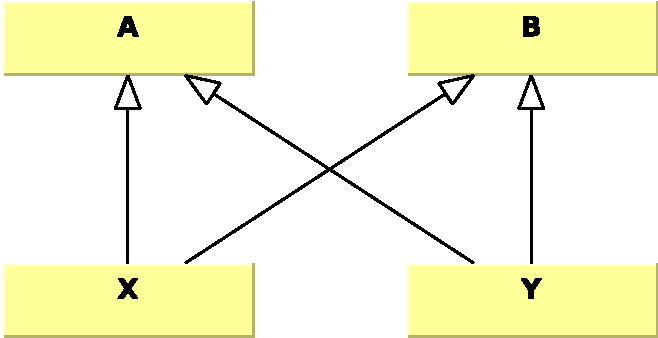
\includegraphics[width=0.4\textwidth]{figures/multiple-inheritance-problem.pdf}
		\caption{One of the problems with type inference in case of multiple inheritance}
		\label{fig:multiple-inheritance-problem}
	\end{center}
\end{figure}

If the types of the variables are known then the types of the parameters can be inferred. 
For this, we collect the variables that represent this parameter from each body.
As the parameters value can be any of the variable, we choose the type, that generalizes them.
If no such type exists, the inference of the parameter type is failed.

We also maintain additional information in our representation. 
Bodies also maintain the relationship between variables and parameters. 
In PSystem, this information is not directly available, parameters and variables need to be matched by name.

\section{Search plan calculation}

\subsection{Creating a basic plan}
After we have extended PSystem with the needed information, we can plan how the pattern will be evaluated at runtime, i.e.\ how the query code will process the graph and produce matches for the pattern.

The first step is flattening and normalization. 
The purpose of flattening is to replace pattern calls with the constraints of the bodies of the referenced pattern, as in most of the cases this leads more efficient code, than handling the pattern as a black box.
At normalization, equality constraints are optimized: equal variables are unified, and equality constraint is omitted.

After flattening and normalization, we need to create the search plan for each body of the pattern. From a set of constraints that declaratively defines the body we need to create an imperative sequence of search operations.

For this, we use the local search planner of \viatra{}.
This planner takes a pattern and a cost function, then creates a permutation of constraints that minimizes the cost function. 
The cost function gives an approximated cost of applying a constraint based on the variables bound before the application and other information\footnote{One of the used detail is the statistics on the instance model: As it can only be available at runtime, we can't use these at design time}. 
After this permutation is achieved, then search operations will be created by mapping the constraints to them considering their position.

For the different types of constraint applications we use the following search operations. We also give the basic search operation a name to use them later in the examples.


\subsubsection{Equality and pattern find}
These two types of constraints are never appear in this phase, as they are both optimized. Pattern find constraints are replaced with their inner constraints in the flattening phase, while Equality constraints are optimized in normalization phase.


\subsubsection{Type constraint}
We apply a type constraint the following way:

\begin{itemize}
\item If the variable is bound, we need to check whether the already bound value is of that type, we denote this CheckInstanceOf(Var, Type).
\item If the variable is unbound, we need to iterate over the instances of the type and follow the algorithm, we denote this ExtendInstanceOf(Var, Type) ).
\end{itemize}


\subsubsection{Reference and attribute (Structural feature) constraint}

Reference and attribute relations are called structural features.
We apply the constraint of a structural feature the following way:
\begin{itemize}
	\item If the source and target variable is bound too, then we just checks, whether the constraint is satisfied by those constraint. 
	
	\mbox{(CheckNavigation(from, to, structural feature))}
	\item If the source variable is bound and the target is unbound, then we extend along using the source variable for all its elements (or single element, if it does not have multiplicity). 
	
	\mbox{(ExtendNavigation(from, to, structural feature))}
	\item If the target variable is bound and the source is unbound, then we check, if the structural feature is a reference having an opposite reference. 
	\begin{itemize}
		\item If it is, then we can navigate along the opposite reference, so we can use it to extend to the source variable. 
		
		\mbox{ExtendNavigation(to, from, opposite structural feature)}
		\item If not, we add two search operation: 
		
		ExtendInstanceof(type of src, src), CheckNavigation(src, target). 
	\end{itemize}

	\item If both of  target variable and the source is unbound, then we use the next 2 search operation: ExtendInstanceof(type of src, src), ExtendNavigation(src, target)

\end{itemize}


\subsubsection{Negative pattern call and transitive closure}

We only apply these constraints, when all the referred variables are bound, so we only compile them into check operations:
\begin{itemize}
	\item Negative pattern application $\rightarrow{}$ NegativePatternCheck(pattern, $v_1$, $v_2$, \dots{} )
	\item Transitive closure $\rightarrow{}$ BinaryTransitiveClosureCheck(pattern, $v_1$, $v_2$).
\end{itemize}

\subsubsection{Count pattern matches}

This constraint can be applied, when all the variables given to the sub pattern as parameter are bound. 
The count of the matches is stored in another variable. 
We choose the search operation based on this variable.

\begin{itemize}
	\item If this variable is bound, then we create a check operation: 
	CheckPatternMatchCounter(countVar, pattern, $v_1$, $v_2$, \dots{})
	\item If this variable is not bound, then we create an extend operation: 
	ExtendPatternMatchCounter(countVar, pattern, $v_1$, $v_2$, \dots{})
\end{itemize}


\subsubsection{Inequality}
Inequality is only supported as a check operation: CheckInequality(x, y)


\subsection{Expanding the plan for distributed evaluation}
Now the sequence of search operation can be used to find the matches of a pattern on a single computer, but in a distributed setup, we need additional steps to make the plan correct.
The following search operations can cause problems in a distributed setup:
\begin{itemize}
	\item CheckNavigation	
	\item ExtendNavigation
	\item ExtendInstanceOf
\end{itemize}

CheckNavigation and ExtendNavigation need the source object to be available at the computing unit, because references and attributes are stored on local objects.
ExtendInstanceOf needs to expa

\subsubsection{Example for search plan creation on a pattern }
\todo{examplet csinálni ide}


\subsection{Additional optimization}

After we complete the plan with type information and other details, it can be used to generate C++ code, although before that step we use further optimizations. 
These optimizations considers distributed execution of the plan, so it can improve the plan generated by \viatra{} which is generated to be used in a single computer.


\subsubsection{Replace pattern calls with simpler operations}
There are some cases, where helper patterns are simple, and used to define simple conditions. 
In this case, evaluationg the subquery is not always the most efficient method, sometimes these can be replaced by simple search operations:

\paragraph{Reference Pattern}
We use the phrase \emph{reference pattern} for a pattern with 2 parameters if its only constraint is that a reference exist between the two parameters, eg.:
\begin{lstlisting}[language = vql]
private pattern connected(a : RailRoadElement, b : RailRoadElement){
	RailRoadElement.connectedTo(a,b);
}
\end{lstlisting}

In the following examples i will use this query as an example to demonstrate how the application of this query can be replaced by an other operation.

\paragraph{Counting reference pattern} 
Instead of counting a reference pattern bounding the source variable, we can insert a search operation counting the references.

\begin{lstlisting}[language = vql]
1 == count find connected(a, _);
\end{lstlisting}


\paragraph{Negative application of a reference pattern}
Instead of checking wether a reference pattern matches we can simply create a search operation which checks the existence of the reference.
\begin{lstlisting}[language = vql]
neg find connected(a, _);
\end{lstlisting}

\todo{Lesz itt egy összefoglaló táblázat ezekről mindről}


\subsubsection{Filter unnecessary operations, checks}
As the original plan is generated by the localsearch planner of \viatra{}, there can be redundant operations, which can be ommited. This includes:

\begin{itemize}
	\item Check operation -- The generated code is strongly typed, so we don't need type checks in most cases, unlike in the Java implementation, where the tuples contains plain java objects with unknown types.
	
	\item Distribution operations -- We also need to detect redundant distribution operations, this can happen, when we know, that a certain object is local after the previous operation.
\end{itemize}



\section{\protect\cpptt{} code generation}



\subsection{Generated code structure}

The structure of the generated code is depicted on \autoref{fig:generated-code-structure-perpattern}.
For each pattern we generate a \texttt{Matcher} class.
This class contains the methods for query execution.
We also generate a \texttt{Match} class which is a data class for pattern match.
A \texttt{MatchSet} class is also generated which holds a subresult of a query, which is a collection of matches.
We generate \texttt{Frame} classes, which can holds variable bindings. 
Since different parameter-bound patterns and different bodies of a pattern can contain a different set of variables, we generate multiple frame class for a pattern.


\begin{figure}[h]
	\begin{center}
		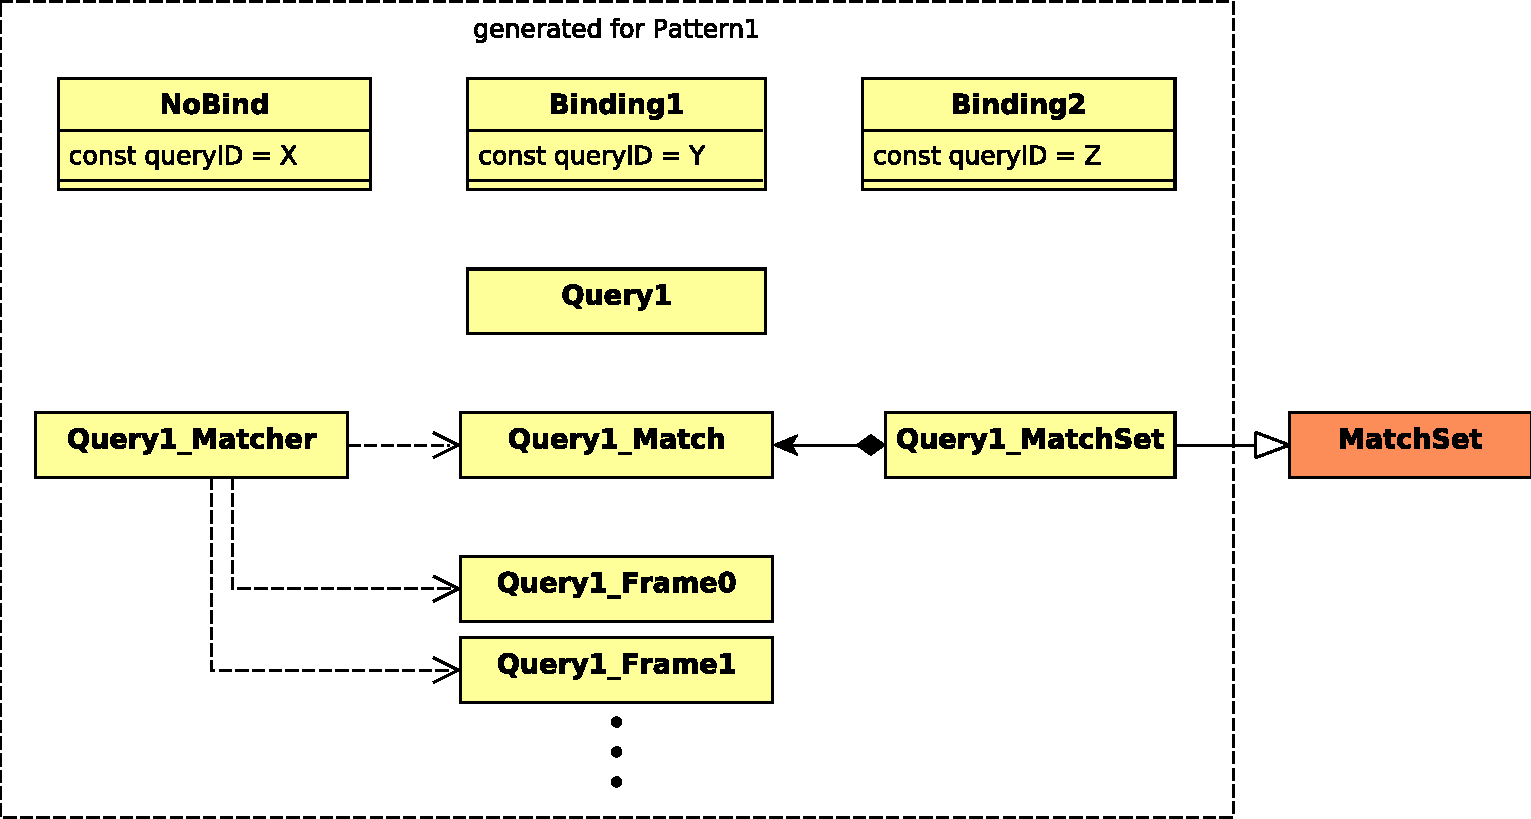
\includegraphics[width=\textwidth]{figures/generated-code-structure-perpattern.pdf}
		\caption{Generated classes for a pattern}
		\label{fig:generated-code-structure-perpattern}
	\end{center}
\end{figure}


\subsection{Integrating with the framework}

\begin{figure}[h]
	\begin{center}
		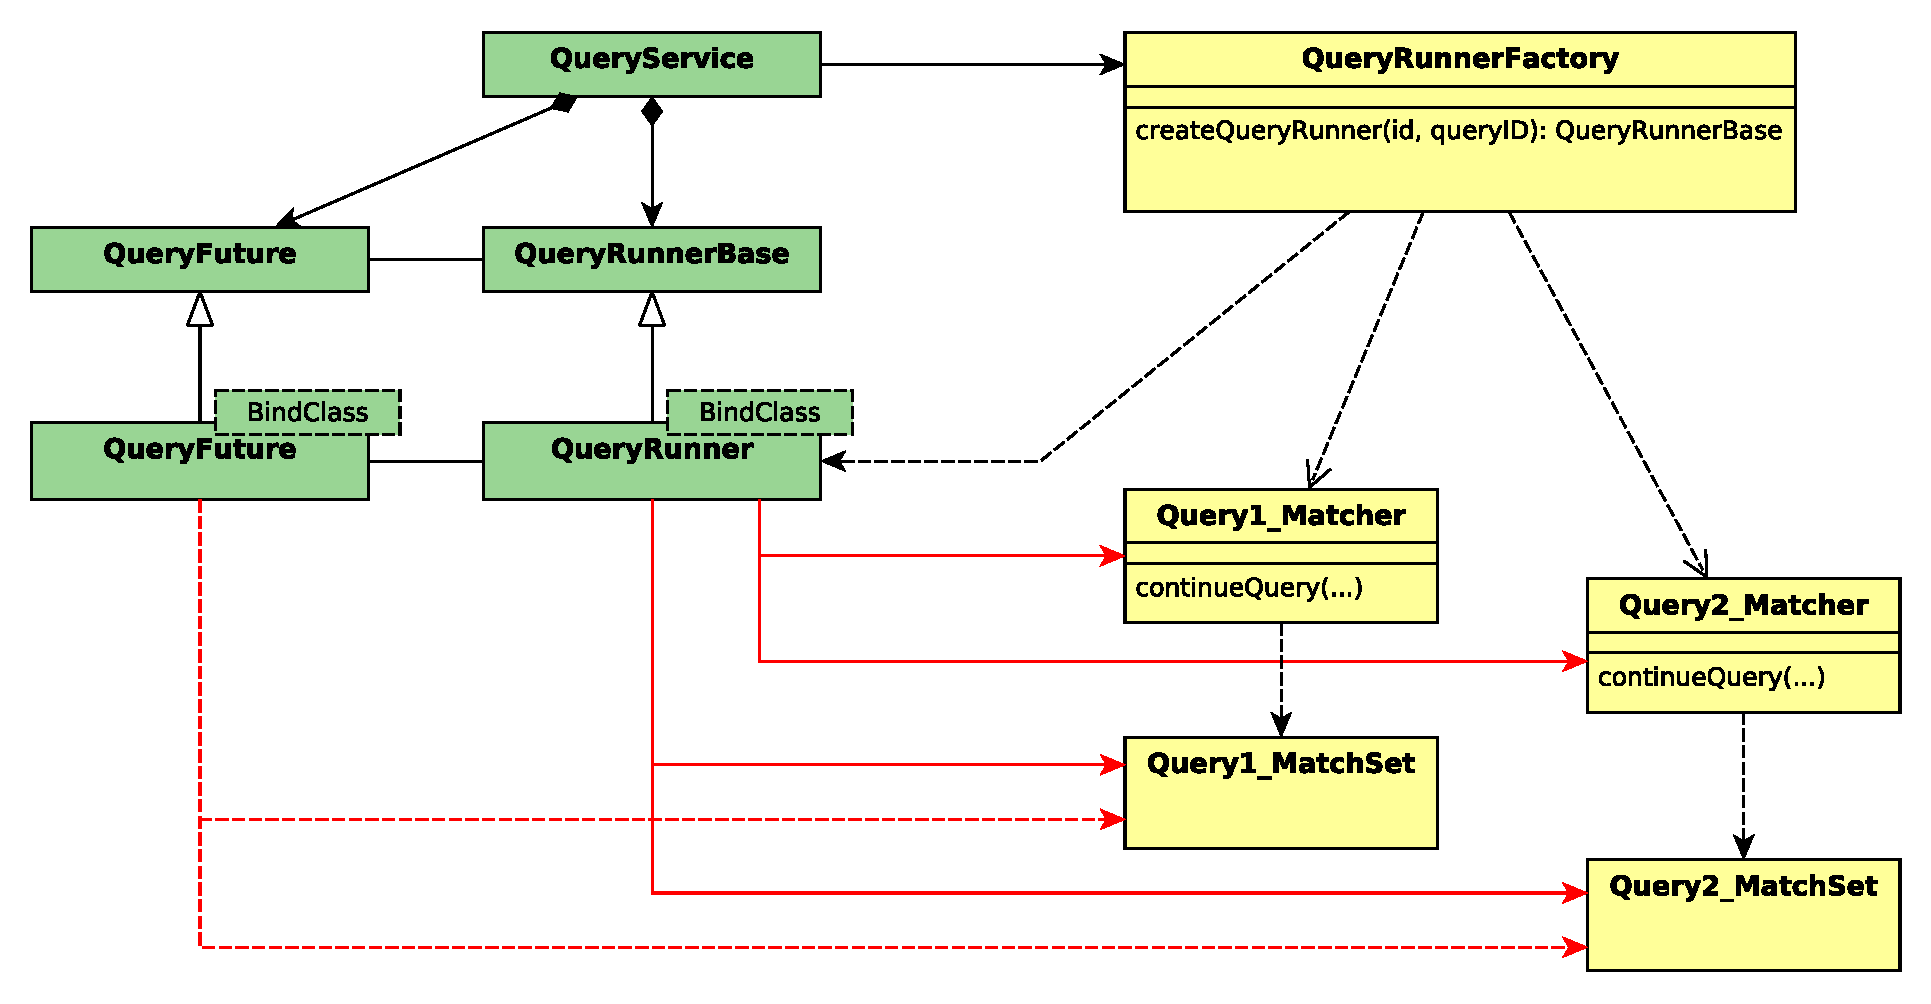
\includegraphics[width=0.7\textwidth]{figures/generated-code-structure-wholesome.pdf}
		\caption{Generated code structure for every pattern}
		\label{fig:generated-code-structure-wholesome}
	\end{center}
\end{figure}

\subsection{Query code generation}

The completed and optimized plan are used to generate \cpp{} code. 
Two main methods can be used to run local search plan in case of generated code. 
One is to generate the plan as a data structure and create an interpreter that uses the plan to find matches. 
The other is to generate the code directly from the plan. 
The first method is good if we want to change the plan at runtime, but the interpreter itself introduces an overhead, causing performance to be slower.
We implemented and measured the performance for both of them.

\todo{Itt konkrétan a kódgenerálás részleteibe bele lehet menni, ha lesz idő}


\subsection{Generating helper data structures}

\subsubsection{Matching frame, frame vector}

The variables of a body are stored in a data structure called the matching frame.
We also generate a collection for frames called frame vector used in distributed behavior of the graph pattern matcher.
We generate serializer and deserializer methods, which uses protobuf.
The message structure (.proto file) is also generated alongside these structures.
\todo{Konkrétan megcsinálni, hogy hogy generálódnak az osztályok, adattagok, névválasztás, XXXMAtchingFrame0, stb}

\subsubsection{Match, MatchSet}

These are used to store graph pattern matches. Match is a singular match (Practically it is the same as the Matching Frame projected to the parameters), while MatchSet is a collection for matches.













